% [Claude] 2026-11-05 (user request): Fig. 2b on the real scenes. tests/plot_scene_avg_coef.py -> plots/scene_avg_coef/avg_blending_weight_
% {nvidia,dycheck}_sorted.pdf (copied to img/): average softmax blending weight per basis, ours (split_init at the tables' B) vs SoM-10, mean over
% seeds 42-44 (block SoM: 42 / 43), each run's bases sorted by weight; rank k averaged over the scenes that have it (ours: NVIDIA 7 7 7 7 6 5 2 1,
% DyCheck 5 5 5 5 5 4 4 4 3 1). Curves: NVIDIA ours 0.372 0.244 0.174 0.104 0.070 0.043 0.037 0.034, SoM-10 0.190 0.158 0.133 0.112 0.097 0.087
% 0.074 0.058 0.050 0.042; DyCheck ours 0.375 0.183 0.123 0.087 0.072 0.069 0.054 0.042 0.037 0.038, SoM-10 0.182 0.146 0.122 0.111 0.102 0.087
% 0.075 0.068 0.060 0.046 (top values to 4 decimals: 0.3719 / 0.1897 NVIDIA, 0.3746 / 0.1824 DyCheck).
% [Claude] 2026-11-05: NVIDIA panel switched from native to sorted order (user request), restored after a concurrent edit reverted it.
\begin{figure}[t]
  \centering
  \begin{subfigure}{\linewidth}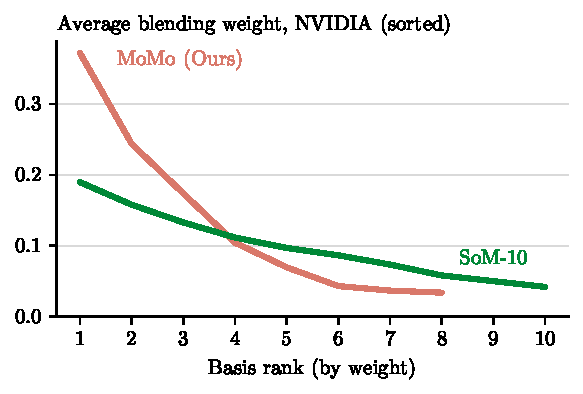
\includegraphics[width=\linewidth]{img/avg_blending_weight_nvidia_sorted.pdf}\phantomsubcaption\label{fig:avg-weight-nvidia}\end{subfigure}\\[2pt]
  \begin{subfigure}{\linewidth}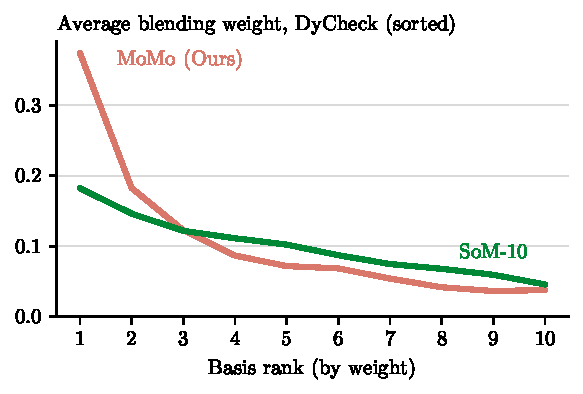
\includegraphics[width=\linewidth]{img/avg_blending_weight_dycheck_sorted.pdf}\phantomsubcaption\label{fig:avg-weight-dycheck}\end{subfigure}
  \caption{Average blending weight of each basis on the real scenes: ours with the
    $B$ its stopping rule picks per scene against SoM~\cite{wang2025shape} with its default 10 bases (SoM-10), mean over three seeds and
    over the scenes, with each model's bases sorted by weight, which does not depend on SoM's arbitrary basis order. Top: the seven
    NVIDIA scenes. Bottom: the five DyCheck scenes. A rank is averaged over the scenes that have it, so ours ends at the largest $B$ of
    the dataset.}
  \label{fig:avg-weight-real}
\end{figure}
